\documentclass[main]{subfiles}

\begin{document}
    \section{Сложность, присущая программному обеспечению. Оценки сложности алгоритмов и представления данных}
    Известный специалист в области программного проект Брукс:\\
    "Эйнштейн утверждал, что должны существовать простые объяснения природных процессов, т.к. Бог не действовал по капризу или произволу. У программиста нет такого утешения: сложность, с которой он должен справиться, лежит в самой природе системы."{}\\

    Почему программному обеспечению присуща сложность? Это связано с:
    \begin{enumerate}
        \item Сложностью реальной предметной области, из которой исходит заказ на разработку
        \item Трудностью управления процессом разработки (много разработчиков, функция сложности управления проектов — примерно факториал числа участников, если только пары — примерно квадрат)
        \item Необходимостью обеспечить достаточную гибкость программы (много параметров и противоречивость требований)
        \item Эволюцией программного обеспечения
        \item Неудовлетворительными способами описания поведения больших дискретных систем
    \end{enumerate}
    Последним мы можем в какой-то мере управлять. Для уменьшения сложности ПО используют метод декомпозиции. Декомпозиция – внесение порядка в сложную систему.\\

    Существует два типа декомпозиции:
    \begin{enumerate}
        \item Алгоритмическая декомпозиция --- разделение системы, путем разделения алгоритмов, где каждый модуль системы выполняет один из этапов общего процесса (внимание на порядок событий)
        \item Объектно-ориентированная (ОО) декомпозиция --- выбрав в качестве критерия декомпозиции принадлежность ее элементов к различным абстракциям данной проблемной области. Абстракции описываются в виде объектов. Тогда каждый объект обладает своим собственным поведением, и каждый из них моделирует некоторый объект реального мира. С этой точки зрения объект является вполне осязаемой вещью, которая демонстрирует вполне определенное поведение. Объекты что-то делают, и мы можем, послав им сообщение, попросить их выполнить то-то и то-то (концентрируя внимание на агентах, действующих в предметной области)
    \end{enumerate}

    С чего лучше начинать и почему? Важны оба способа декомпозиции, но лучше начинать проектирование с ОО декомпозиции.
    \begin{enumerate}
        \item ОО декомпозиция уменьшает размер программных систем за счет повторного использования общих механизмов и программных компонентов — существенно экономит выразительность средств
        \item ОО системы более гибки и проще эволиционируют со временем, т.к. их схемы базируются на устойчивых формах; большие системы развививаются из маленьких, уже проверенных
        \item (проще анализ), поскольку улучшается структура программного проекта, например, иерархическая структура
    \end{enumerate}

    Дополнительные источники сложности:
    \begin{enumerate}
        \item Научно-практическая проблема, которую следует решить
        \item Существующая (применяемая) технология реализации решения
    \end{enumerate}

    \subsection{Методы оценки сложности алгоритмов}
    Пусть $n \in \N$ — наиболее существенный параметр некоторой задачи или код нескольких таких параметров задачи, например, номер кортежа этих параметров в некоторой нумерации. И пусть требуется оценить время (дискретное) работы алгоритма, решающего эту задачу или объем памяти (в некоторых единицах памяти), требуемых для решения этой задачи при неограниченном увеличении значения параметра.\\

    Единицы измерения могут быть абстрактным или (псевдо)конкретными.\\

    При этом "время"{} или "память"{} оцениваются как некоторая функция $f$ от данного параметра $n$.

    \begin{definition}
        Эту функцию иногда называют мерой или функцией сложности задачи.
    \end{definition}

    \begin{definition}
        Пусть даны неотрицательные функции: $f$ — функция сложности и $g$ — функция, называемая оценкой сложности.
        \[f(n) = O(g(n)) \LRA \e c > 0 \q \e k \q \forall n \geq k \q f(n) \leq c \cdot g(n)\]
        \[f(n) = O(g(n)) \LRA \e c > 0 \q \e k \q \forall n \geq k \q f(n) \geq c \cdot g(n)\]
        \[f(n) = O(g(n)) \LRA \e a,b > 0 \q \e k \q \forall n \geq k \q a \cdot g(n) \leq f(n) \leq b \cdot g(n) \text{, где $g$ --- "точная"{} оцнка $f$}\]
    \end{definition}
    Примеры. Гамильтонов цикл графа $О(n*n!)$, выполнимость булевской формулы – $NP$-полные.\\

    Гамильтонов граф — математический объект теории графов. Представляет собой граф (набор точек и соединяющих их линий), который содержит гамильтонов цикл. При этом гамильтоновым циклом является такой цикл (замкнутый путь), который проходит через каждую вершину данного графа ровно по одному разу.\\

    Обычно оценку сверху получают для всех возможных значений параметра, даже самых "плохих"{}, поэтому часто эти оценки наз "оценки в худшем случае"{}.\\

    "в среднем"{}, "в лучшем случае"{}\\
    Однако также для самых интересных или часто встречающихся значений параметра находят оценки "в среднем"{} (быстрая сорт.), а иногда, редко, и "в лучшем случае" (снизу). Это необходимо всегда оговаривать.
    \begin{figure}[H]
        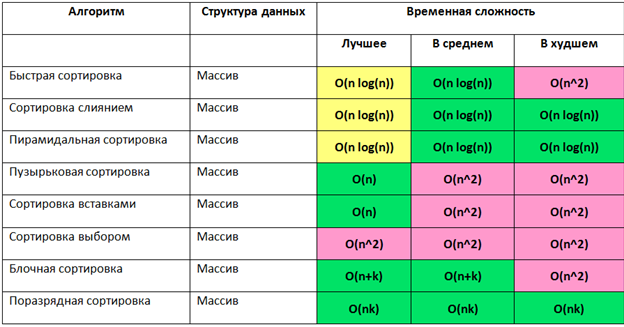
\includegraphics[width = 13cm]{pics/2_1}
        \centring
    \end{figure}
    Графы
    \begin{figure}[H]
        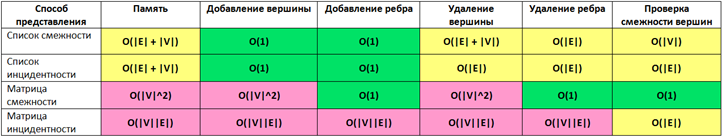
\includegraphics[width = 13cm]{pics/2_2}
        \centring
    \end{figure}
\end{document}
